%Correct the file name.
%X: book number
%Y: part number
%ZZZ: page number in three digits. So page 3 would be 003.

\documentclass[11pt]{amsbook}

\usepackage{../HBSuerDemir}	% ------------------------


\begin{document}

% ++++++++++++++++++++++++++++++++++++++
\hPage{b1p2/334}
% ++++++++++++++++++++++++++++++++++++++
$$\sigma_{n} = \epsilon_{1} \dotsc \epsilon_{n} = 1 . $$
\begin{exmp}
Proves the nth roots of unity can be represented as powers of $\epsilon\left(=\epsilon_1\right)$ as$$\epsilon,\epsilon^2,\dotsc,\epsilon^n$$
\end{exmp}
\begin{proof}
Since $\epsilon_k=\cos\ k  \frac{2\pi}{n}+i\ \sin\ k  \frac{2\pi}{n}$ and $\epsilon=\cos\ \frac{2\pi}{n}+i\ \sin\ \frac{2\pi}{n}$,
from De Moivre's formula, we have
$$\epsilon_k=\ \left(\cos\ \frac{2\pi}{n}+i\ \sin\ \frac{2\pi}{n}\ \right)^k=\epsilon^k,\quad k=1,\dotsc,n.$$
\end{proof}
\section{EXERCISES (4.4)}

\begin{enumerate}
    \item[66.] Find $\hAbs{z}$ and Arg z for the following complex numbers : \\
    a) $-3+i$ \qquad b) \ $1-\sqrt{3}i$\qquad c) \ $-3i$\qquad\ \qquad  d)\ $7$
    \item[67.]Show that $i^n=i^r$ if $n=r$ \quad $\left(mod 4\right)$
    \item[68.]Write the polar form of: \\
    a) \ $3-3i$ \qquad b) $2+2\sqrt{3}i$\qquad c)\ $3\sqrt{3}-3i$\qquad d)\ $-5$
    \item[69.]Find the polar form of the product of the complex numbers \\
    $z_1=2+i$ and $z_2=3+i$ without finding their product.
    \item[70.]Find the polar form of the ratio $\left(3-i\right)/\left(1-3i\right)$ of two complex numbers without performing the division.
    \item[71.]Sketch the following loci of points: \\
    a)$\left\{z: \hAbs{z}=2,\quad  z \in \epsilon \right\}$, \qquad
    b)$\left\{z: \frac{\hAbs{z-1}}{\hAbs{z-2i}}=1,\quad  z \in \epsilon \right\}$
    \item[72.]Same question for: \\
    a)$\left\{z: \hAbs{z}>3,\quad  z \in \epsilon \right\}$, \qquad
    b)$\left\{z: \frac{\hAbs{z-1}}{\hAbs{z-2}}=\frac{1}{2},\quad  z \in \epsilon \right\}$
    \item[73.]Sketch the following sets in Arg and plane: \\
    a)$\left\{z: 1<\hAbs{z}<4, z \in \epsilon \right\}$, \qquad 
    b)$\left\{z: \hAbs{z-1}+\hAbs{z+1}=3, z \in \epsilon \right\}$
\end{enumerate}

% =======================================================
\end{document}  

%==== templates ====

%==== environments ====

%\begin{figure}[htb]
%	\centering
%	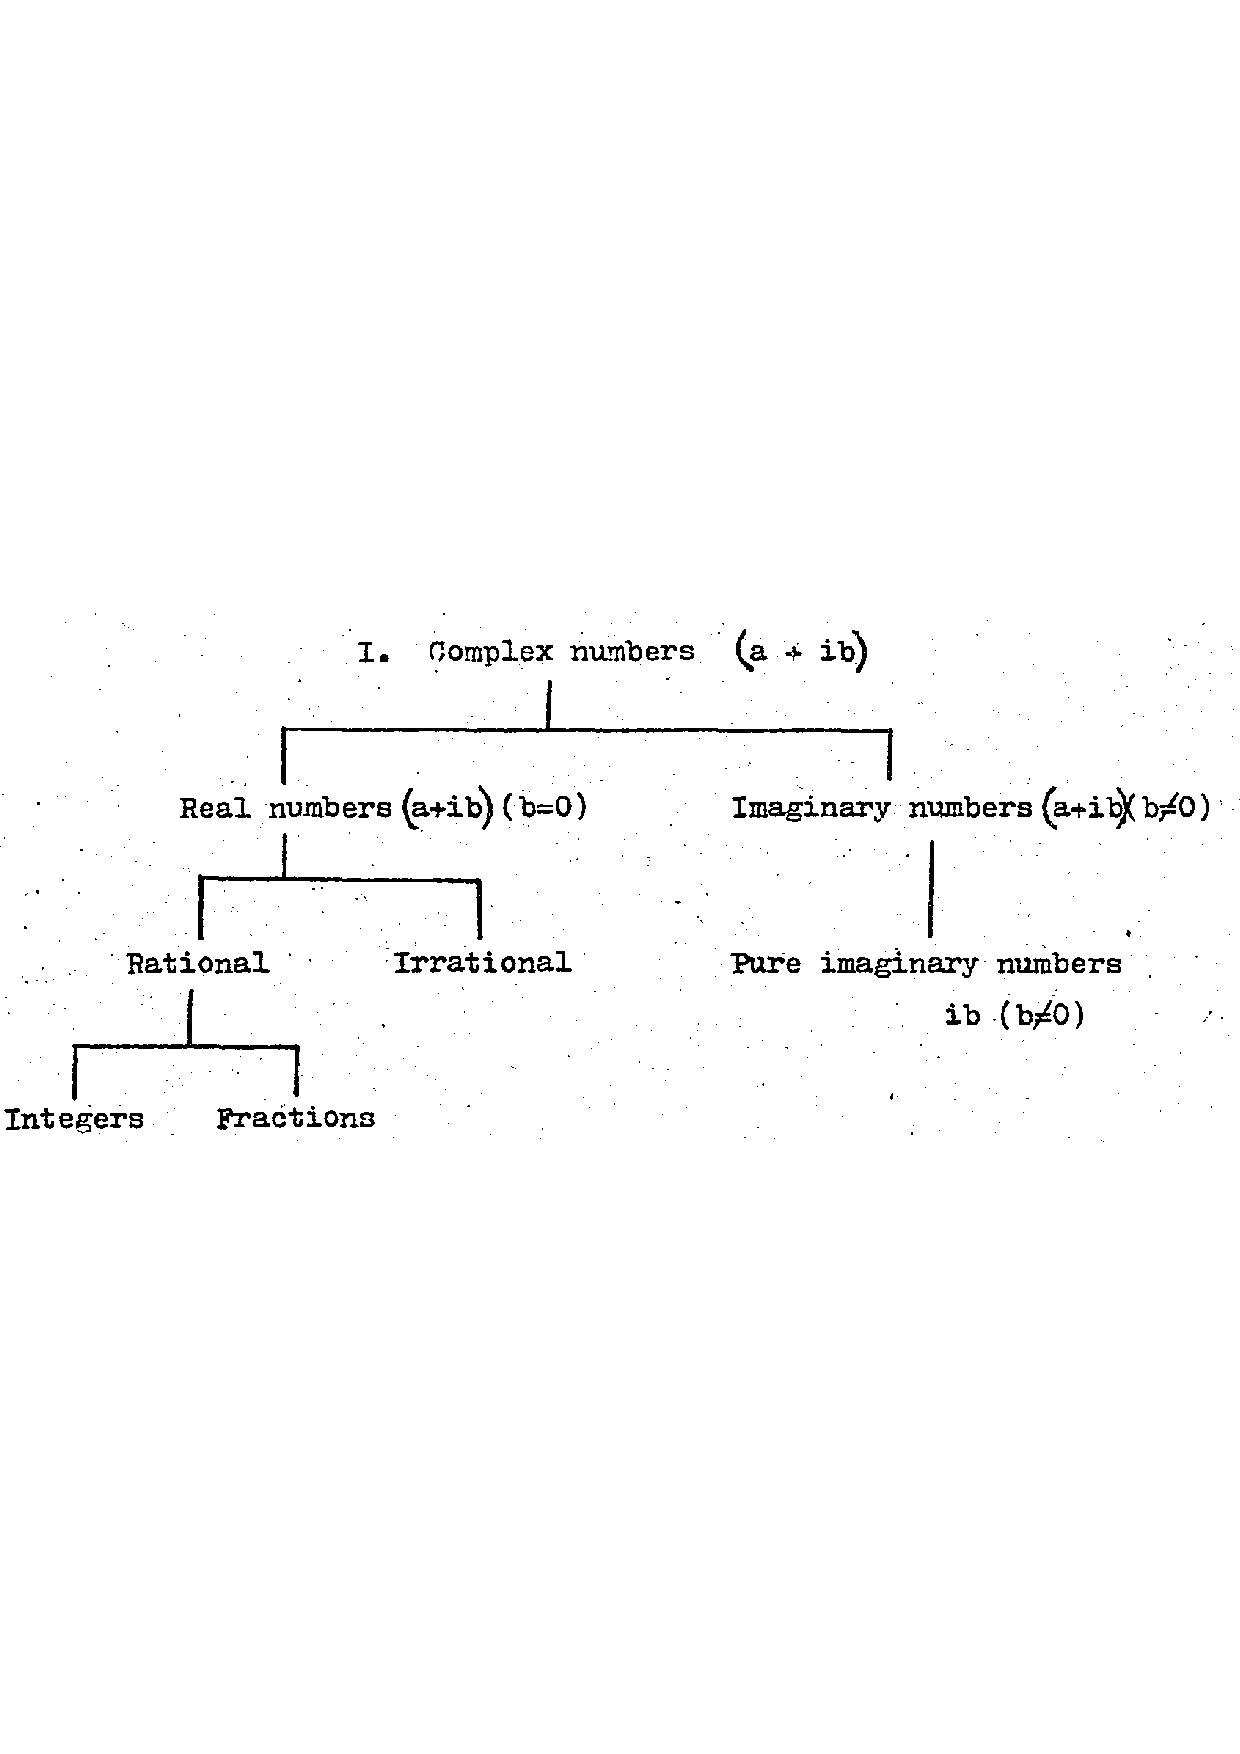
\includegraphics[width=0.9\textwidth]{images/SD-1-1p15A}
%	\caption{Classification of complex numbers}
%	\label{fig:classificationOfComplexNumbersA}
%\end{figure}

%\begin{center}
%\begin{tabular}{cc}
%\end{tabular}
%\end{center}

%\begin{exmp}
%\begin{hSolution}
%\end{hSolution}
%\end{exmp}

%\begin{hEnumerateAlpha}
%\end{hEnumerateAlpha}

%\begin{hEnumerateRoman}
%\end{hEnumerateRoman}

%$
%\begin{bmatrix}
%\end{bmatrix}
%$

%\frac{aaaa}{bbb}
%\frac{a_{n}}{b_{n}}
%\left( aaaa \right)
%\Longrightarrow

%\begin{multicols}{2}
%	bb
%\columnbreak
%	aa
%\end{multicols}
